\documentclass[border=10pt]{standalone}
\usepackage{amsmath}
\usepackage{tikz}
\usetikzlibrary{arrows.meta,angles,quotes,calc}
\definecolor{acc}{HTML}{0D9488}
\definecolor{ink}{HTML}{1A1D21}
\definecolor{mut}{HTML}{646A72}
\begin{document}
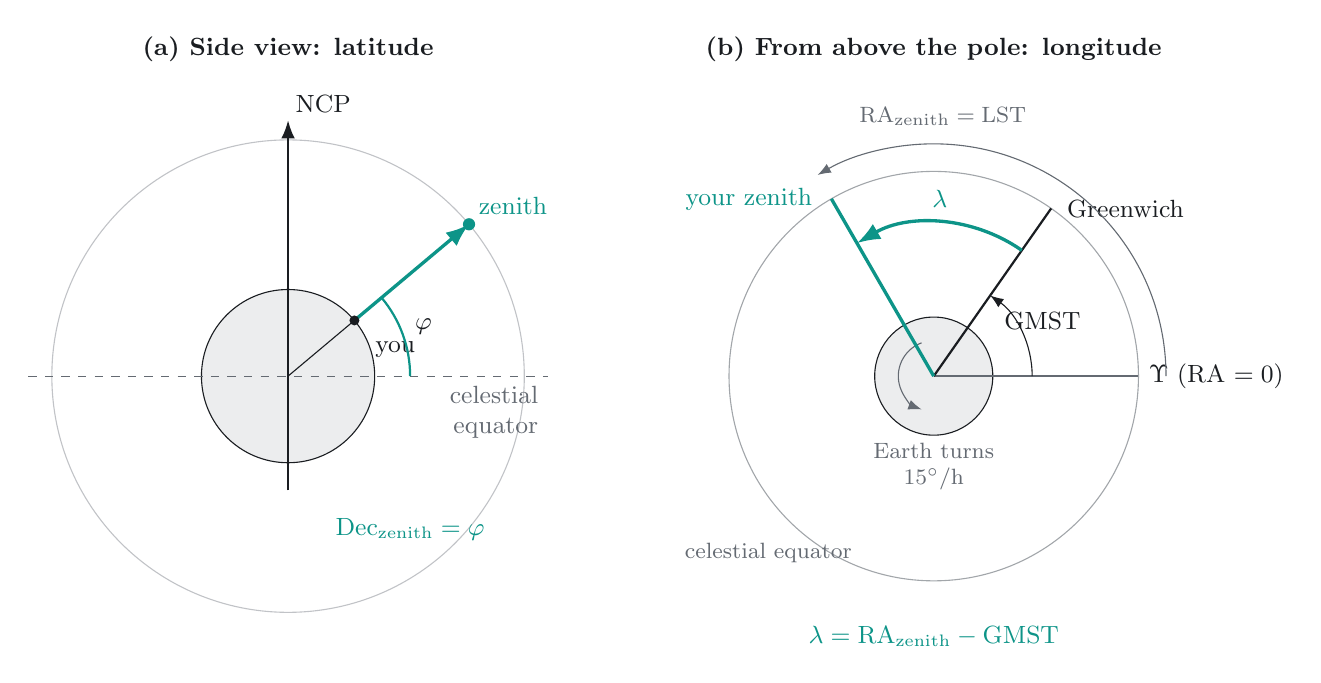
\begin{tikzpicture}[>=Latex, font=\small, every node/.style={text=ink}]
  % (a) side view in the observer's meridian plane
  \begin{scope}
    \node[font=\bfseries\small] at (0,4.15) {(a) Side view: latitude};
    \draw[mut!40] (0,0) circle (3);
    \fill[mut!12] (0,0) circle (1.1);
    \draw[ink] (0,0) circle (1.1);
    \draw[->, ink, thick] (0,-1.45) -- (0,3.25) node[above right=-1pt] {NCP};
    \draw[dashed, mut] (-3.3,0) -- (3.3,0) node[below left, align=right, text=mut] {celestial\\equator};
    \coordinate (O) at (0,0);
    \coordinate (E) at (3,0);
    \coordinate (Z) at (40:3);
    \coordinate (P) at (40:1.1);
    \draw[acc, very thick, ->] (P) -- (Z);
    \fill[acc] (Z) circle (2.2pt) node[above right, text=acc] {zenith};
    \draw[ink] (O) -- (P);
    \fill[ink] (P) circle (1.8pt) node[below right=4pt] {you};
    \draw[acc, thick] pic["$\varphi$", draw, angle radius=1.55cm, angle eccentricity=1.18] {angle=E--O--Z};
    \node[align=center, text=acc] at (1.55,-1.95) {$\mathrm{Dec}_{\text{zenith}} = \varphi$};
  \end{scope}
  % (b) view from above the north celestial pole
  \begin{scope}[xshift=8.2cm]
    \node[font=\bfseries\small] at (0,4.15) {(b) From above the pole: longitude};
    \draw[mut!60] (0,0) circle (2.6);
    \node[text=mut, font=\footnotesize] at (-2.1,-2.25) {celestial equator};
    \fill[mut!12] (0,0) circle (0.75);
    \draw[ink] (0,0) circle (0.75);
    \draw[->, mut] (110:0.45) arc (110:250:0.45);
    \node[text=mut, font=\footnotesize, align=center] at (0,-1.15) {Earth turns\\$15^\circ$/h};
    \coordinate (O) at (0,0);
    \coordinate (A) at (0:2.6);
    \coordinate (G) at (55:2.6);
    \coordinate (L) at (120:2.6);
    \draw[mut, thick] (O) -- (A) node[right] {$\Upsilon$ (RA $= 0$)};
    \draw[ink, thick] (O) -- (G) node[right=2pt] {Greenwich};
    \draw[acc, very thick] (O) -- (L) node[left=3pt, text=acc] {your zenith};
    \draw[ink, ->] (0:1.25) arc (0:55:1.25);
    \node at (27:1.55) {GMST};
    \draw[acc, very thick, ->] (55:1.95) arc (55:120:1.95);
    \node[text=acc] at (88:2.25) {$\lambda$};
    \draw[mut, ->] (0:2.95) arc (0:120:2.95);
    \node[text=mut, font=\footnotesize] at (88:3.3) {$\mathrm{RA}_{\text{zenith}} = \mathrm{LST}$};
    \node[text=acc] at (0,-3.3) {$\lambda = \mathrm{RA}_{\text{zenith}} - \mathrm{GMST}$};
  \end{scope}
\end{tikzpicture}
\end{document}
